\documentclass[12pt]{beamer}
\usepackage[latin1]{inputenc}
\usetheme{Madrid}

\title[Economics 6330\hspace{2em}\insertframenumber/
\inserttotalframenumber]{DATA 5600 -- Introduction to Regression for Data Analytics}

\author[Brough]{Tyler J. Brough}
\institute[USU]{
  Department of Economics and Finance \\
  Jon M. Huntsman School of Business \\
  Utah State University \\
}
\date{\today}
\begin{document}

\begin{frame}
\titlepage
\end{frame}


\section{Agenda for 03/21/2022}
%------------------------------ slide ----------------------------------%
\begin{frame}
\frametitle{Agenda for Today}
\begin{itemize}
 \item Brief Review of Statistical Inference
 \item Discuss further topics in Mathematical Statistics:
 \begin{itemize}
  \item Large sample properties of estimators
  \item Confidence intervals
  \item Hypothesis testing
 \end{itemize}
\end{itemize}
\end{frame}


\section{Brief Review of Some Concepts}
%------------------------------ slide ----------------------------------%
\begin{frame}
\frametitle{The Normal Distribution}
The normal probability density function is defined as follows:

\vspace{5mm}
\begin{equation*}
f(x) = \frac{1}{\sigma \sqrt{2\pi}} \exp{\frac{-(X-\mu)^{2}}{2\sigma^{2}}}, \quad \mbox{for $-\infty < x < \infty$}
\end{equation*}

\vspace{5mm}
where $E(X) = \mu$ and $Var(X) = \sigma^{2}$. When a random variable is normally distributed we write 
$X \sim N(\mu, \sigma^{2})$.
\end{frame}


%------------------------------ slide ----------------------------------%
\begin{frame}
\frametitle{The Normal Distribution}
A special case is the standard normal distribution, which is defined as follows:

\begin{equation*}
\phi(z) = \frac{1}{\sqrt{2\pi}} \exp\left\{\frac{-z^{2}}{2}\right\}, \quad \mbox{for $-\infty < z < \infty$} 
\end{equation*}

\vspace{5mm}
The standard normal cumulative distribution function is denoted by $\Phi(z) = P(Z \leq z)$. Using some basic 
facts from probability we arrive at the following helpful formulas:

\begin{align*}
P(Z > z)  &= 1 - \Phi(z) \\
P(Z < -z) &= P(Z > z) \\
P(a \leq Z \leq b) &= \Phi(b) - \Phi(a)
\end{align*}
\end{frame}


%------------------------------ slide ----------------------------------%
\begin{frame}
\frametitle{The Chi-Square Distribution}
The chi--square distribution is obtained directly from independent, standard normal random variables.
Let $Z_{i}$, $i = 1, 2, \ldots, n$, be independent random variables, each distributed as standard normal. Define a
new random variable as the sum of the squares of the individual $Z_{i}$:

\vspace{5mm}
\begin{equation*}
X = \sum\limits_{i=1}^{n} Z_{i}^{2}
\end{equation*}

\vspace{5mm}
The new random variable $X$ has a chi--square distribution with $n$ degrees of freedom. This is 
often written as $X \sim \chi_{n}^{2}$.
\end{frame}


%------------------------------ slide ----------------------------------%
\begin{frame}
\frametitle{The Student $T$ Distribution}
The $t$ distribution is a workhorse in classical statistics and econometrics. A $t$ distribution is
obtained from a standard normal and a chi--square random variable. Let $Z$ have a standard normal distribution
and let $X$ have a chi-square distribution with $n$ degrees of freedom. Also assume that $Z$ and $X$ are independent.
Then the following random variable

\vspace{5mm}
\begin{equation*}
T = \frac{Z}{\sqrt{X/n}}
\end{equation*} 

\vspace{5mm}
has a $t$ distribution with $n$ degrees of freedom. This is denoted by $T \sim t_{n}$. The $t$ distribution gets
its degrees of freedom from the chi--square random variable.
\end{frame}


%------------------------------ slide ----------------------------------%
\begin{frame}
\frametitle{The $F$ Distribution}
Another important distribution for statistics and econometrics is the $F$ distribution. To define an $F$
random variable, let $X_{1} \sim \chi_{k_{1}}^{2}$ and $X_{2} \sim \chi_{k_{2}}^{2}$ and assume that $X_{1}$ and
$X_{2}$ are independent. Then, the random variable

\begin{equation*}
F = \frac{X_{1}/k_{1}}{X_{2}/k_{2}}
\end{equation*}

has an $F$ distribution with $(k_{1}, k_{2})$ degrees of freedom. We denote this as $F \sim F_{k_{1}, k_{2}}$. The 
order of the degrees of freedom is important. $k_{1}$ is the \emph{numerator degrees of freedom} and $k_{2}$ is 
the \emph{denominator degrees of freedom}.
\end{frame}


\section{Mathematical Statistics}
%------------------------------ slide ----------------------------------%
\begin{frame}
\frametitle{Large Sample Properties of Estimators}
We saw with the estimator of $\mu$, $W = Y_{1}$ that it was an unbiased, but poor estimator. One notable
feature of $Y_{1}$ is that its variance is the same no matter what its sample size. It is reasonable to 
require that as the $\left[n \rightarrow \infty \mbox{,} \quad \sigma^{2} \rightarrow 0\right]$ sample size increases
the estimation procedure improves.

\vspace{5mm}
Example: $\bar{Y}$ for estimation of population mean $\mu$

\begin{equation*}
s^{2} = Var(\bar{Y}) = \frac{1}{n-1} \sum\limits_{i=1}^{n} (Y_{i} - \bar{Y})^{2}
\end{equation*}

\vspace{5mm}
As $n \rightarrow \infty$, $s^{2} \rightarrow 0$.
\end{frame}


%------------------------------ slide ----------------------------------%
\begin{frame}
\frametitle{Consistency}
Let $W_{n}$ be an estimator of $\theta$ based on a sample $Y_{1}, Y_{2}, \ldots, Y_{n}$ of size $n$. Then
$W_{n}$ is a \emph{consistent estimator} of $\theta$ if for every $\epsilon > 0$

\vspace{2mm}
\begin{equation*}
P(|W_{n} - \theta| > \epsilon) \rightarrow 0 \quad \mbox{as} \quad n \rightarrow \infty
\end{equation*}

\vspace{3.5mm}
If $W_{n}$ is not consistent for $\theta$, we say it is \emph{inconsistent}. When $W_{n}$ is consistent,
we also say that $\theta$ is the probability limit of $W_{n}$, written as 

\begin{equation*}
plim(W_{n}) = \theta
\end{equation*}

\vspace{3.5mm}
Interpretation:

\begin{itemize}
 \item[] The distribution of $W_{n}$ becomes more and more concentrated about $\theta$, which means
         that for larger sample sizes, $W_{n}$ is less and less likely to vary far from $\theta$.
\end{itemize}
\end{frame}


%------------------------------ slide ----------------------------------%
\begin{frame}
\frametitle{Python Simulation to Show Consistency}
\begin{itemize}
 \item Go to Python, then come back.
 \item See code \emph{lln.py} in course repo
\end{itemize}
\end{frame}


%------------------------------ slide ----------------------------------%
\begin{frame}
\frametitle{The Law of Large Numbers}
Let $Y_{1}, Y_{2}, \ldots, Y_{n}$ be independent, identically distributed random variables with mean
$\mu$. Then

\vspace{2mm}
\begin{equation*}
plim(\bar{Y}) = \mu
\end{equation*}

\vspace{3.5mm}
Interpretation:

\begin{itemize}
 \item[] If we want to estimate the population average $\mu$, we can get arbitrarily close to $\mu$ by
         choosing a sufficiently large sample.
\end{itemize}
\end{frame}


%------------------------------ slide ----------------------------------%
\begin{frame}
\frametitle{Properties of the Probability Limit}
\textbf{Propery PLIM1:} \\

\vspace{3mm}
Let $\theta$ be a parameter and define a new parameter $\gamma = g(\theta)$, for some continuous function
$g(\theta)$. Suppose that $plim(W_{n}) = \theta$. Define an estimator $\gamma$ by $G_{n} = g(W_{n})$. Then
$plim(G_{n}) = \gamma$.

\vspace{3mm}
Often stated as: $plim(g(W_{n})) = g(plim(W_{n}))$ for a continuous function $g(\theta)$.

\vspace{3mm}
Example: $g(\theta) = a + b \theta$, $g(\theta) = \sigma^{2}$, $g(\theta) = \frac{1}{\theta}$,
         $g(\theta) = \sqrt{\theta}$, $g(\theta) = \exp{\theta}$.
\end{frame}


%------------------------------ slide ----------------------------------%
\begin{frame}
\frametitle{Properties of the Probability Limit}
\textbf{Property PLIM2:} \\

\vspace{5mm}
If $plim(T_{n}) = \alpha$ and $plim(U_{n}) = \beta$ then

\begin{itemize}
 \item[(i)]   $plim(T_{n} + U_{n}) = \alpha + \beta$
 \item[(ii)]  $plim(T_{n}U_{n}) = \alpha \beta$
 \item[(iii)] $plim\left(\frac{T_{n}}{U_{n}} \right) = \frac{\alpha}{\beta}$, for $\beta \neq 0$
\end{itemize}

\end{frame}


%------------------------------ slide ----------------------------------%
\begin{frame}[shrink=10]
\frametitle{An Example}
Example: Let $\left\{Y_{1}, Y_{2}, \ldots, Y_{n} \right\}$ be a random sample of size $n$ an annual
earnings from the population of workers with a high school education with population mean $\mu_{Y}$.

\vspace{2mm}
Let $\left\{Z_{1}, Z_{2}, \ldots, Z_{n} \right\}$ be a random sample of size $n$ on annual earnings 
from the population of workers with a college education with population mean $\mu_{Z}$.

\vspace{2mm}
We wish to estimate the percentage difference in annual earnings between the two groups, which is
$\gamma = 100 \frac{(\mu_{Z} - \mu_{Y})}{\mu_{Y}}$, the percentage by which earnings for college 
grads differs from high school grads.

\vspace{2mm}
Because $\bar{Y}$ is consistent for $\mu_{Y}$, and $\bar{Z}_{n}$ is consistent for $\mu_{Z}$ it follows
that 

\vspace{2mm}
\begin{equation*}
G_{n} = 100 \frac{(\bar{Z}_{n} - \bar{Y}_{n})}{\bar{Y_{n}}} 
\end{equation*}

\vspace{2mm}
is a consistent estimator of $\gamma$.
\end{frame}


%------------------------------ slide ----------------------------------%
\begin{frame}
\frametitle{Asymptotic Normality}
Let $\left\{Z_{n}: n = 1, 2, \ldots \right\}$ be a sequence of random variables, such that for all 
numbers $Z$

\begin{equation*}
P(Z_{n} \leq z) \rightarrow \Phi(z) \quad \mbox{as} \quad n \rightarrow \infty
\end{equation*}

\vspace{2mm}
in which $\Phi(z)$ is the standard normal CDF. $Z_{n}$ is said to have an asymptotic standard normal
distribution. 

\vspace{2mm}
Asymptotic normality holds for large $n$, we have the approximation $P(Z_{n} \leq z) \approx \Phi(z)$. 
This means that probabilities concerning $Z_{n}$ can be approximated by the standard normal probabilities.
\end{frame}


%------------------------------ slide ----------------------------------%
\begin{frame}
\frametitle{The Central Limit Theorm}
\vspace{2mm}
Let $\left\{Y_{1}, Y_{2}, \ldots, Y_{n} \right\}$ be a random sample with mean $\mu$ and variance 
$\sigma^{2}$. Then

\begin{equation*}
Z_{n} = \frac{\bar{Y} - \mu}{\sigma/\sqrt{n}}
\end{equation*}

\vspace{2mm}
has an asymptotic standard normal distribution.
\end{frame}



%------------------------------ slide ----------------------------------%
\begin{frame}
\frametitle{Confidence Interval Estimation}
A \emph{Confidence Interval} is a range of values, calculated from the sample observations,
that are believed, with a particular probability, to contain the true parameter value.
\end{frame}

%------------------------------ slide ----------------------------------%
\begin{frame}[shrink=20]
\frametitle{An Example of Confidence Interval Estimation}
Example:

\vspace{2mm}
Suppose the population has a $N(\mu, \sigma = 1)$ distribution and let 
$\left\{Y_{1}, Y_{2}, \ldots, Y_{n} \right\}$ be a random sample from this
population (assume $\sigma = 1$ known).

\vspace{2mm}
The sample average $\bar{Y}$ has a normal distribution with mean $\mu$ and variance
$\frac{1}{n}$

\begin{equation*}
\bar{Y} \sim N\left( \mu, \frac{1}{n} \right)
\end{equation*}

\vspace{2mm}
Standardizing $\bar{Y}$ which will give it a standard normal distribution

\begin{equation*}
P \left( -1.96 < \frac{\bar{Y} - \mu}{1/\sqrt{n}} < 1.96 \right) = 0.95
\end{equation*}

\vspace{2mm}
Tells us that the probability that the random interval 
$[\bar{Y} - 1.96/\sqrt{n}, \bar{Y} + 1.96/\sqrt{n} ]$, contains the population mean $\mu$
is $0.95$ or $95\%$.
\end{frame}

\section{Confidence Intervals}
%------------------------------ slide ----------------------------------%
\begin{frame}
\frametitle{Confidence Interval Estimation}
\vspace{2mm}
This allows us to construct an interval estimate of $\mu$

\begin{equation*}
[\bar{y} - 1.96/\sqrt{n}, \quad \bar{y} + 1.96/\sqrt{n} ]
\end{equation*}

This is called a $95\%$ confidence interval. This is denoted as $\bar{y} \pm 1.96/\sqrt{n}$.
\end{frame}


%------------------------------ slide ----------------------------------%
\begin{frame}
\frametitle{Confidence Interval Estimation}
\vspace{2mm}
Example: suppose $n = 16$ and $\bar{y} = 7.3$ then

\vspace{3mm}
\begin{equation*}
7.3 \pm 1.96/\sqrt{16} = 7.3 \pm 0.49 = [6.81 \mbox{,} 7.79]
\end{equation*}
\end{frame}

%------------------------------ slide ----------------------------------%
\begin{frame}
\frametitle{Confidence Interval Estimation}
\vspace{2mm}
Interpretation: the random interval $[\bar{Y} - 1.96/\sqrt{n} \mbox{,} \quad \bar{Y} + 1.96/\sqrt{n}]$
contains $\mu$ with probability $0.95$.

\vspace{2mm}
In other words, if we sampled from the population and calculated the random interval infinitely
many times, it would contain the population parameter $\mu$ $95\%$ of the time.

\vspace{2mm}
Note: It does not mean: $P(\bar{Y} - 1.96/\sqrt{n} \leq \mu \leq + 1.96/\sqrt{n}) = 0.95$ 
because parameters $\theta$ are \textit{not} variables. 
\end{frame}

%------------------------------ slide ----------------------------------%
\begin{frame}
\frametitle{Confidence Interval Estimation}
\begin{itemize}
 \item Python simulation exercise to show confidence intervals.
 \item See Python code \emph{interval.py} in course repo
\end{itemize}
\end{frame}


%------------------------------ slide ----------------------------------%
\begin{frame}
\frametitle{The Confidence Interval for the Mean of a Normal Population}
\vspace{2mm}
Assume $X \sim N(\mu, \sigma)$ and $\sigma$ is known to be any value, the 
$95\%$ CI is

\vspace{5mm}
\begin{equation*}
[\bar{y} - 1.96 \sigma / \sqrt{n} \mbox{,} \bar{y} + 1.96 \sigma / \sqrt{n} ]
\end{equation*}
\end{frame}


%------------------------------ slide ----------------------------------%
\begin{frame}[shrink=20]
\frametitle{Confidence Interval for the Mean of a Normal Population}
\vspace{2mm}
To  allow for unknown $\sigma$, we must use an estimate. Let

\vspace{2mm}
\begin{equation*}
s = \left( \frac{1}{n-1} \sum\limits_{i=1}^{n} (y_{i} - \bar{y})^{2} \right)^{1/2}
\end{equation*}

\vspace{2mm}
denote the sample standard deviation. Using $s$ for $\sigma$ does not preserve the $95\%$ CI
because we must use the sample to calculate $s$. In this case we will rely on the $t$ 
distribution

\vspace{2mm}
\begin{equation*}
\frac{\bar{Y} - \mu}{S/\sqrt{n}} \sim t_{n-1}
\end{equation*} 

\vspace{2mm}
Where $\bar{Y}$ is the sample average and $s$ is the sample standard deviation of the random sample
$\left\{ Y_{1}, Y_{2}, \ldots, Y_{n} \right\}$. To construct a $95\%$ CI let $c$ denote the $97.5$
percentile in the $t_{n-1}$ distribution.
\end{frame}


%------------------------------ slide ----------------------------------%
\begin{frame}
\frametitle{Confidence Interval for the Mean of a Normal Population}
\begin{figure}[htp]
\centering
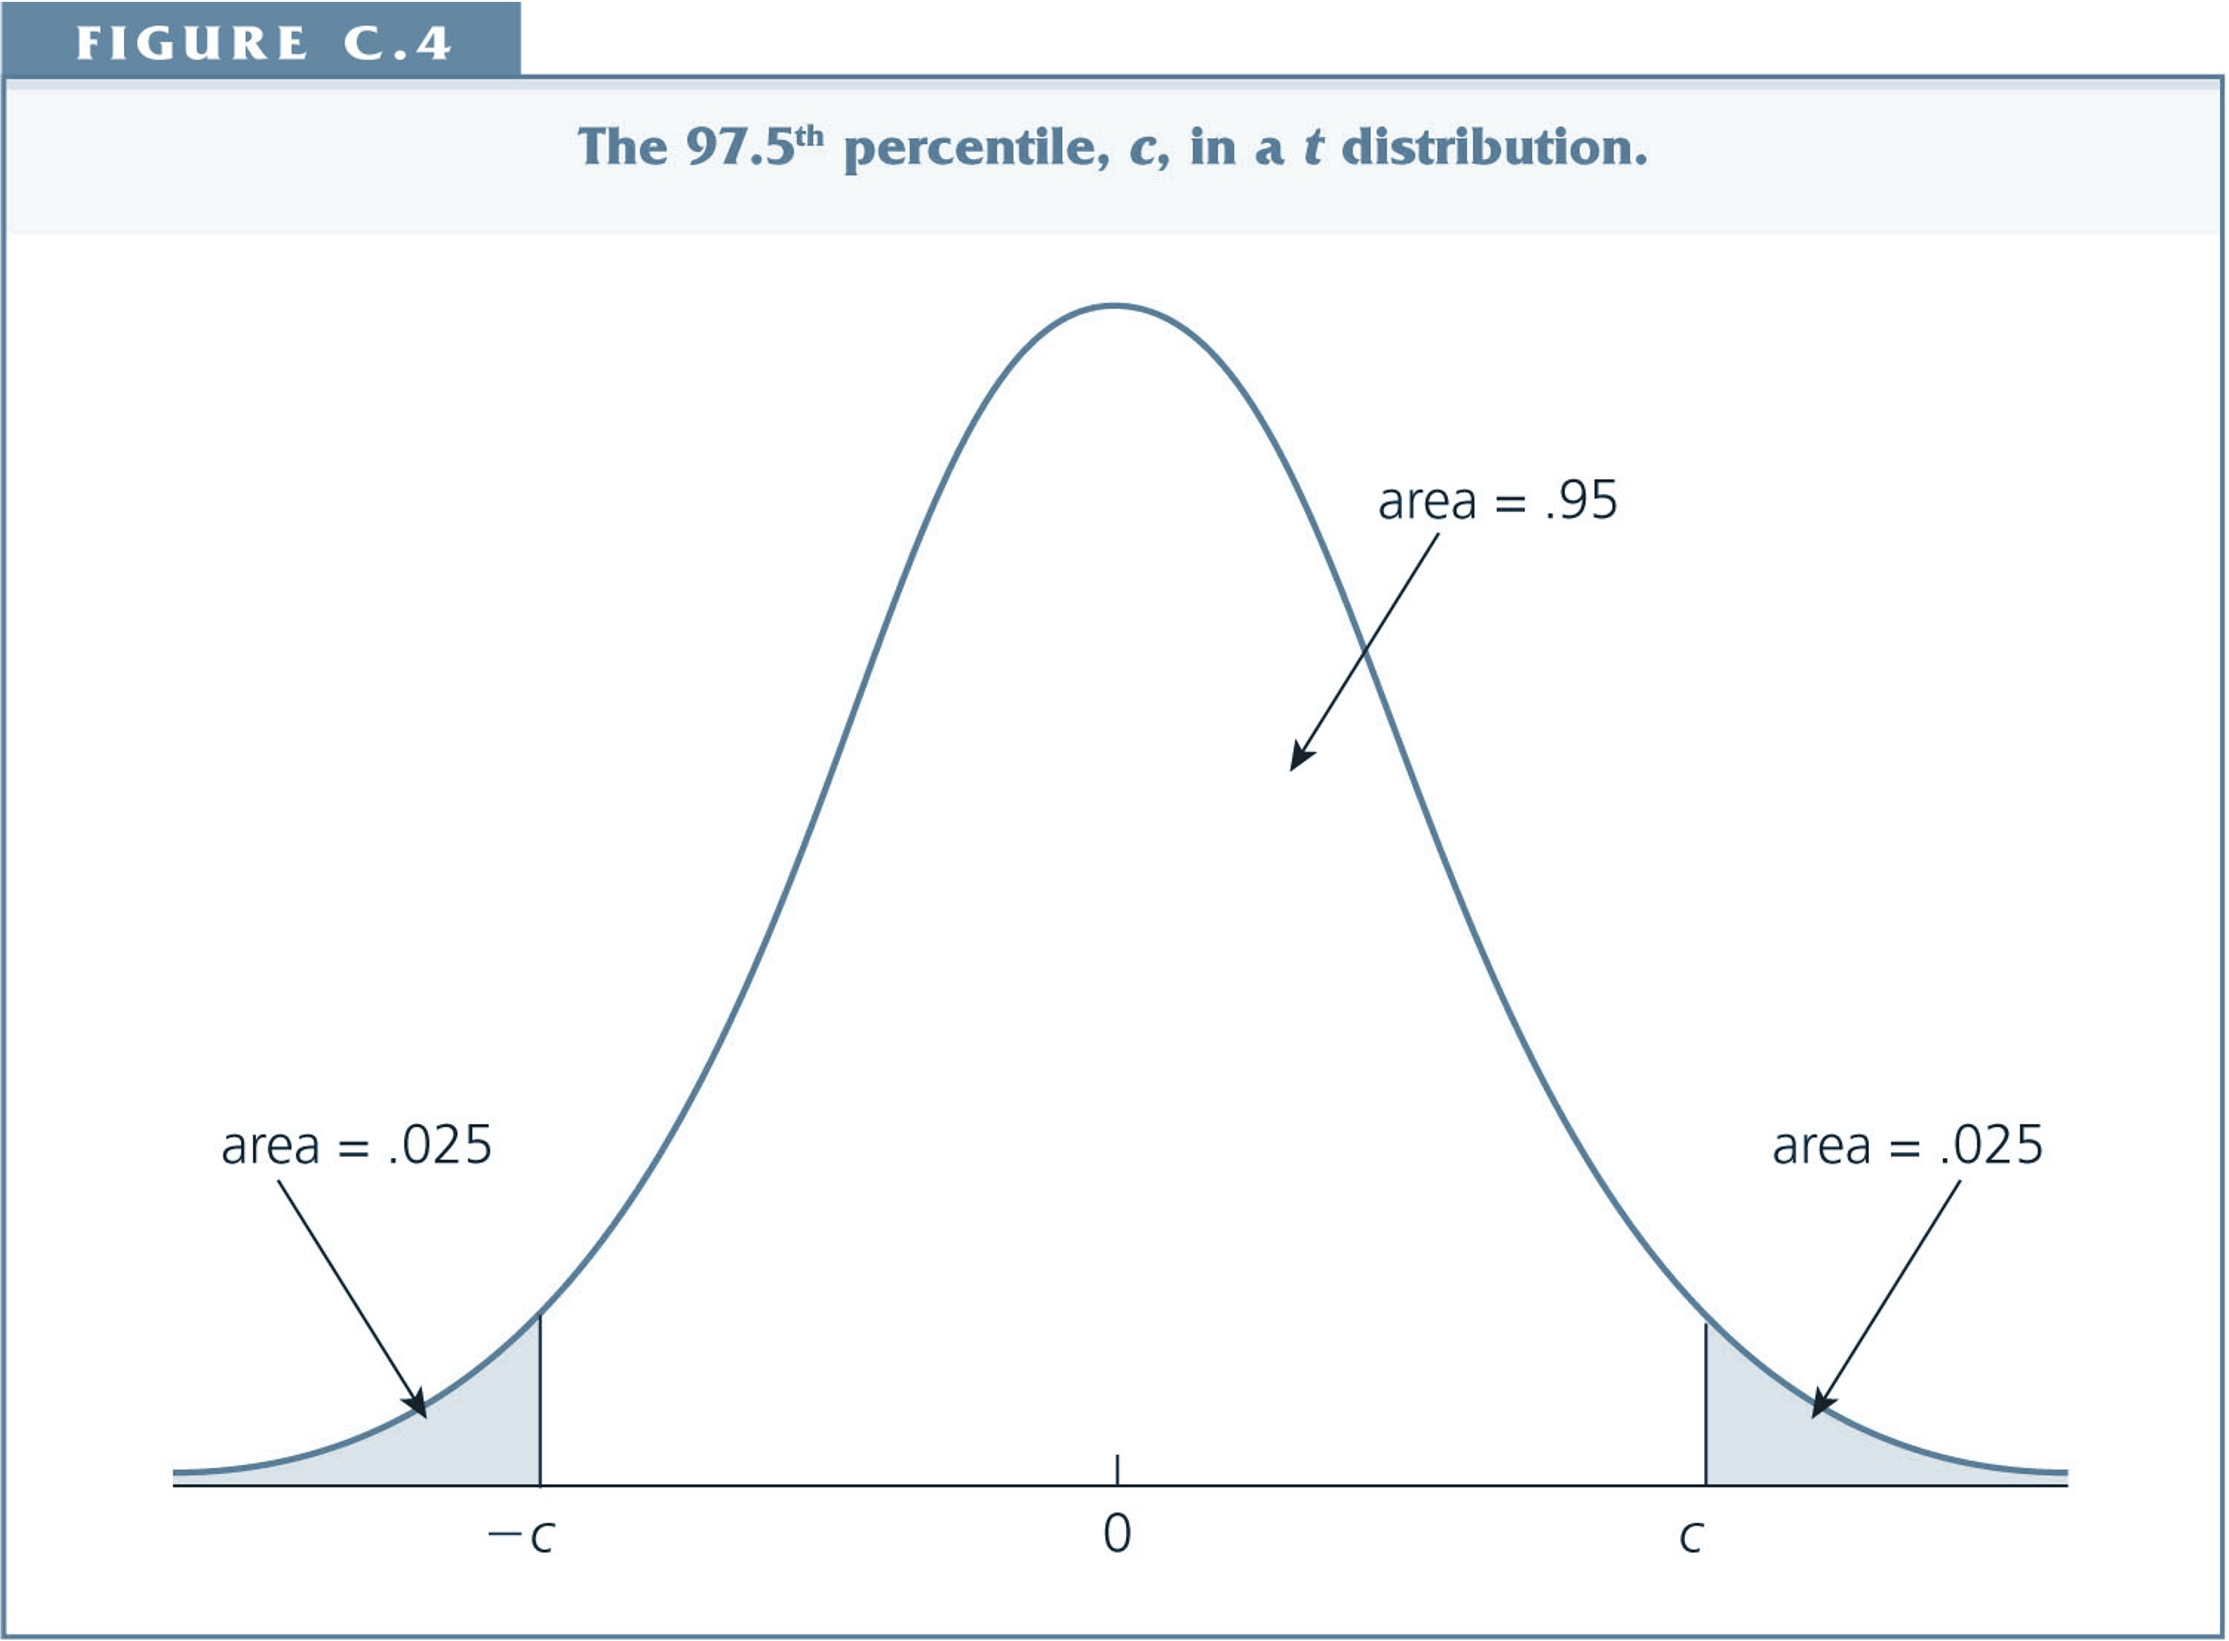
\includegraphics[scale=0.10]{images/FigureC4.jpg}
\end{figure}
\end{frame}

%------------------------------ slide ----------------------------------%
\begin{frame}
\frametitle{Confidence Interval for the Mean of a Normal Population}
In other words:

\begin{equation*}
P(-c < t_{n-1} < c) = 0.95
\end{equation*}

\vspace{2mm}
For a particular sample 

\begin{equation*}
[\bar{y} - c s/\sqrt{n} \mbox{,} \quad \bar{y} + c s/\sqrt{n}]
\end{equation*}

\end{frame}


%------------------------------ slide ----------------------------------%
\begin{frame}
\frametitle{Confidence Interval for the Mean of a Normal Population: Example}
Example: $c$ is chosen from statistical tables for the $t_{n-1}$ distribution. If $n=20$ then
the $df = 20 - 1 = 19$ Then we have $c = 2.093$ and thus

\vspace{2mm}
\begin{equation*}
[\bar{y} \pm 2.093 (s / \sqrt{20}) ]
\end{equation*}

\vspace{3mm}
Example: Consider job training grants on worker production. Let

\begin{itemize}
 \item[] $n = 20$
 \item[] $c = 2.093$
 \item[] $\bar{y} = 1.15$
 \item[] $se(\bar{y}) = 0.54$
\end{itemize}
\end{frame}


%------------------------------ slide ----------------------------------%
\begin{frame}
\frametitle{Confidence Interval for the Mean of a Normal Population: Example}
Then we have

\vspace{5mm}
\begin{equation*}
CI_{0.95} = [-2.28 \mbox{,} -0.02]
\end{equation*}

\vspace{5mm}
Interpretation: Zero is excluded. We conclude with $95\%$ confidence that average change
in scrap rates is not zero.
\end{frame}

%------------------------------ slide ----------------------------------%
\begin{frame}
\frametitle{A Simple Rule of Thumb}

A simple rule of thumb for a $95\%$ confidence interval is

\begin{itemize}
 \item The $t$ distribution approaches the Normal distribution as the degrees
       of freedom get large.
 \item In particular for $\alpha=0.05$, $C_{\frac{\alpha}{2}} \rightarrow 1.96$
       as $n \rightarrow \infty$.
 \item An approximate $95\%$ CI is
\end{itemize}

\vspace{3mm}
\begin{equation*}
[\bar{y} \pm z se(\bar{y})]
\end{equation*}

\end{frame}


%------------------------------ slide ----------------------------------%
\begin{frame}
\frametitle{Asymptotic Confidence Intervals for Non-Normal Populations}

\end{frame}



\end{document}





